\documentclass[10pt,a4paper]{article}
\usepackage[latin1]{inputenc}
\usepackage{amsmath}
\usepackage{amsfonts}
\usepackage{amssymb}
\usepackage{graphicx}
\author{Wu Bingzhe}
\title{Extracted the style from the image\\with Deep Neural Network}
\begin{document}
	\maketitle
	\begin{abstract}
		
		In the field of visual art,especially painting,humans have mastered the 
		skill to create unique visual experience through composing a complex interplay
		between the content and style of an image.In other area of computer vision such as object detection and recognition , Convolutional neural networks 
		have recently enjoyed a great success in large-scale image recognition\cite{Krizhevsky2012ImageNet} which has become possible due to large public image repositories,such as ImageNet(Deng et al.,2009),and high-performance computing systems,such as GPUs
		or large-scale distributed clusters\cite{Deng2012Large}(Dean et al.2012).In this project ,we use 
		a neural representations to separate and recombine content and style of arbitrary images.This work also offers a algorithmic understanding of how
		humans create and perceive artistic imagery.
	\end{abstract}
	
	% no keywords
	
	
	
	
	% For peer review papers, you can put extra information on the cover
	% page as needed:
	% \ifCLASSOPTIONpeerreview
	% \begin{center} \bfseries EDICS Category: 3-BBND \end{center}
	% \fi
	%
	% For peerreview papers, this IEEEtran command inserts a page break and
	% creates the second title. It will be ignored for other modes.

	
	
	
	\section{Introduction}
	% no \IEEEPARstart
	In this project ,we use a most powerful Deep Neural Networks in image processing called Convolutional Neural 
	Networks .When Convolutional Neural Networks are trained on object recognition,they develop a representation of the image that makes object
	information increasingly explicit along the processing hierarchy.Therefore,
	along the processing hierarchy of the network,the input image is transformed
	into representations that care about the actual content of the image compared
	to its detailed pixel .In terms of this ,we can directly visualise the information each layer contains about the input image by reconstructing the image 
	only from the feature maps in that layer.High layers in the network capture the high-level content in terms of objects and their arrangement in input image but do not constrain the exact pixel values of reconstruction.In contrast, reconstruction from the lower layers simply reproduce the exact
	pixel values of the original image .In this project ,we refer to the feature 
	responses in high layers of the networks as the content representation\cite{DBLP:journals/corr/GatysEB15a} .
	
	
	To obtain a representation of the style of an input image ,we use a featOn the ure
	space originally designed to capture texture information.This feature space we used is built on top of the filter responses in each layer of the network
	.It consists of the correlations between the different filter responses over the spatial extent of the feature maps.(See Implementation for details).By including the feature correlations of multiple layers,we obatain a multi-scale representation of the input image ,which captures its style information but not the details of content and its arrangement.
	
	Again,we can visualise the information captured bt these style feature spaces built on different layers of the network by construction an image that matches the style representation of a given input image .Indeed reconstruction from the style features from the style features produce 
	texturised versions of the input image that capture its general appearance in 
	terms of color and localised structures.Moreover,the size and complexity of local image structures from the input image increases along the hierarchy,a result that can be explained by the increasing receptive field sizes and feature complexity.We refer to this multi-scale representation as style representation.
	
	In this project ,we can manipulate both representation independently to produce new meaningful image.To demonstrate this work,we generate image mix 
	the content and style representation from two different source images.In particular.
	
	The images are synthesised by finding an image that simultaneously matches the
	content representation of the photograph and the style representation of the
	respective piece of art.While the global arrangement of the original photograph is preserved,the colors and local structures that compose the global scenery are provided by the artwork.Effectively,this renders the photograph in the style of the artwork,such that the apperance of the synthesised image resembles the work of art,even though it shows the same content as photograph.
	
	Of course,image content and style cannot be completly disentangled.When synthesising an image that combine 
	the content of one image whit the style of another image,there usually does not exist an image that perfectly 
	matches both constrains at the same time.However,the loss function we minimise during image synthesis cotains
	two terms for content and style respectively,that are well separated.We can therefore smoothly regulate 
	the emphasis on either reconstructing the content or the style.
	
	In my final project ,we set up an artificial system that achieves a separation
	of image content from style,thus allowing to recast the content of one image in the style of any other image. We demonstrate this by creating new,artistic images that combine the style of several well-known paintings with the content of an arbitrarily chosen photograph that I take.In particular,we derive the neural representations for the content and style of an image from the feature responses of high-performing Deep Neural Networks trained 
	on object recognition.
	
	As outlined above, 
	
	The rest of the report is organized as follows :Section 2 provides a background for CNN and VGG model,and also described the datasets for training model we used.Section 3 presents our described the 
	method we used .Section 4 describes implementation details.Section5 shows our
	experiment result.
	\section{BACKGROUND}
	\subsection{DATASETS}
	ImageNet is a dataset of over 15 million labeled high-resolution images belong to roughly 22,000 categories.The images were collected from teh web and labeled by human labelers using Amazon's Mechanical Turk crowd-sourcing tool.Staring in 2010 ,as part of the Pascal Visual Object Challenge,an annual competition called the ImageNet Large-Scale Visual Recognition Challenge (ILSVRC) has benn held.ILSVRC uses a subset of ImageNet with roughly 1000
	images in each of 1000 categories.In all,there are roughly 1.2 million training images,50,000 validation images,and 150,000 testing images.
	
	ImageNet consists of variable-resolution images,while our system requires a constant input dimensionality .In our training process,we down-sampled the images to a fixed resolution of $256\times 256$.Given a image , we first rescaled 
	the image such that the shorter side was of length 256,and then cropped out the central $256\times 256$ patch from the resulting image.We did not pre
	-process the images in any other way,except for subtracting the mean activity over the training set from each pixel.
	Then we use these picture for 
	training a VGG19(see it in next subsection) model by Caffe\cite{jia2014caffe}(A deeplearning framework).
	
	\subsection{CNN Basics}
	Convolutional neural network (CNN) is first inspired by research in 
	neuroscience.After over twenty years of convolution,CNN has been gaining 
	more and more distinction in research fields,such as computer vision,pattern
	recognition ,NLP.As a classical supervised learning algorithm,CNN employs 
	a feedforward process for recognition and backward path for training.
	
	
	A typical CNN is composed of two components : a feature extractor and a classifier . The feature extractor is used to filter input images into 
	feature maps that represent various features of the image.These features may 
	include corners,lines,circular arch,etc.,which are relatively invariant to
	position shifting or distortions.The output of the feature extractor is a low-dimensional vector containing these features.This vector is then fed into the classifier ,which is usually based on traditional artificial neural 
	networks.The purpose of this classifier is to decide the likelihood of 
	categories that the input image might belong to.
	
	A typical CNN is composed of multiple computation layers.For example,the feature extractor may consist of several convolutional layers and 
	optional sub-sampling layers.Figure 1 illustrates the computation of a convolutional layer.The convolutional layer receives $N$ feature maps as input.Each input feature map is convolved by a shifting window is S,which 
	is normally smaller than K.A totel of M output feature maps will form the 
	set of input feature maps for the next convolutional layer.  
	
	\begin{figure}[h]
		\centering
		{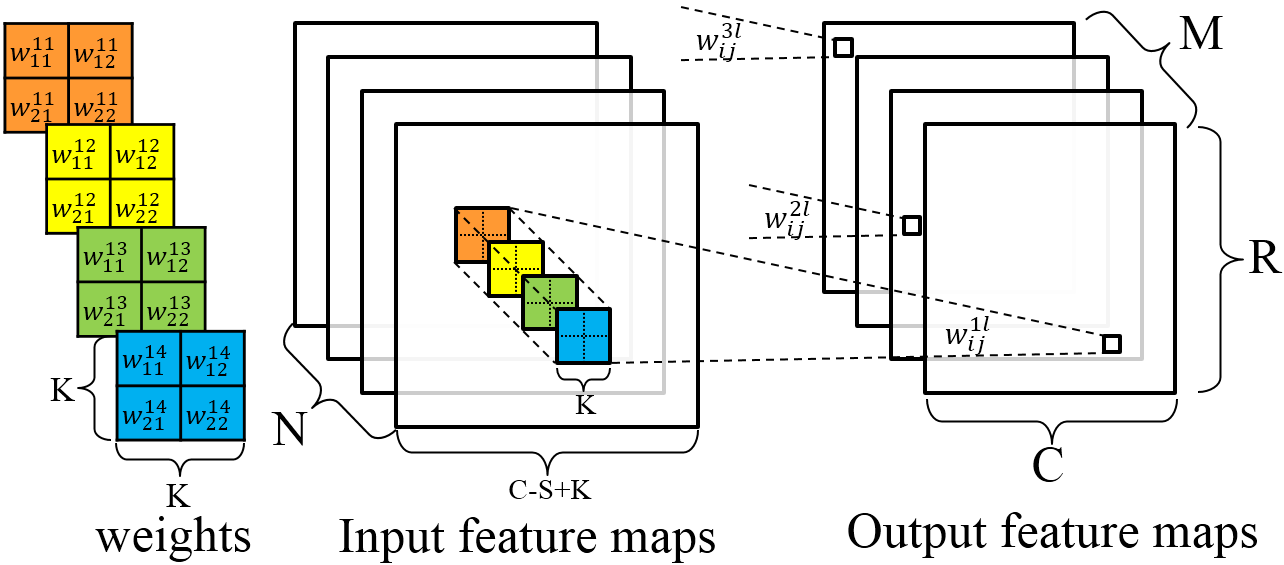
\includegraphics[width=0.8\linewidth]{convolve.png}}
		\caption{Graph of a convolutional layer}
		%	\label{fig_convolve}
	\end{figure}
	\subsection{VGG Model}
	\subsubsection{ARCHITECTURE}
	
	VGG model is a convolutional neural network that rivals human performance 
	on a common visual object recognition benchmark task and was introduced and 
	extensively described in\cite{Simonyan2014Very}. 
	
	In this project ,we used VGG\cite{Simonyan2014Very} models for training.During training,the input
	to this ConvNets is a fixed-size $224\times224$ RGB image.The only pre-processing we do is subtracting the mean RGB value,computed on the training set,from each pixel .The image is passed through a stack of 
	convolution layers,where we use filters with a very small receptive field
	:$3\times 3$(which is the smallest size to capture the notion of left/right,
	up/down,center).In one of the configurations we also utilise $1\times1$ convolution filters,which can be seen as a linear transformation of the
	input channels(followed by non-linearity).The convolutional stride is fixed 
	to 1 pixel ; the spatial padding of conv.layer input is such that the spatial
	resolution is preserved after convolution,i.e.the padding is 1 pixel for $3\times 3$ conv.layers.Spatial pooling is carried out by five max-pooling
	layers,which follow some of the conv.layers(not all the conv.layers are followed by max-pooling).Max-pooling is performed over a $2\times 2$ pixel 
	window,with stride 2.
	
	A stack of convolutional layers (which has a different depth in different 
	architectures) is followed by three Fully-Connected(FC) layers.However in our 
	project ,teh full-connected layers was removed .
	
	All hidden layers are equipped with the rectification(ReLU) non-linearity.
	We note that none of our networks (except for one) contain Local Response
	Normalisation (LRN) normalisation.
	
	The Convnet we used in the project are shown in Figure2
	\begin{figure}[h]
		\centering
		{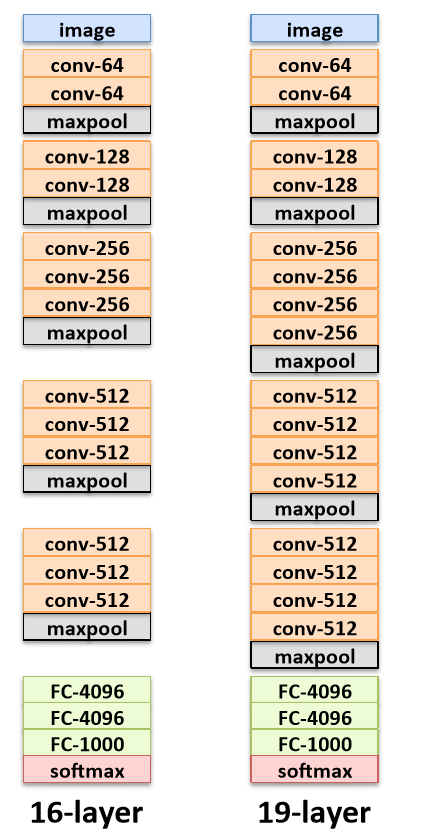
\includegraphics[width=0.8\linewidth]{vgg.png}}
		\caption{Graph of a convolutional layer}
		%	\label{fig_convolve}
	\end{figure}
	\section{Methods}
	The results presented in our project were generated on the basis of 
	the VGG-Model(see details in section 2).We used the feature space provide
	by the 16 convolutional and 5 pooling layers of the 19 layer VGG-Network(
	see the architecture in Figure 2).We do not use any of the fully connected layers.The model is publicly available and can be explored in the caffe-framework. For image synthesis we found that replacing the max-pooling operation by average pooling improves the gradient flow and one obtains slightly more appealing rsults,which is why the images shown were generated 
	whit average pooling.
	
	Generally each layer in the network defines a non-linear filter bank whose 
	complexity increases with the position of the layer in the network .Hence a given input image $\overrightarrow{x}$is encoded in each layer of the CNN by the filter responses to that image.A layer with $N_l$ distinct filters has
	$N_l$ feature maps each of size $M_l$,where $M_l$ is the height times 
	the width of the feature maps. So the responses in a layer $l$ can be stored in a matrix $F^l \in R^{N_l\times M_l}$ where $F_{ij}^{l}$ is the 
	activation of the $i^{th}$ filter at position $j$ in layer $l$.To visualise
	the image information that is encoded at different layers of the hierachy we perform gradient descent on a white noise image to find another image 
	that matches the feature responses of the original image.So let $\overrightarrow{p}$ and $\overrightarrow{x}$ be the original image and the image that is generated and $P^l$ and $F^l$ their respective feature 
	representation in layer $l$.We then define the squared-error loss between the two feature representations :
	\begin{equation}
	L_{content} (\overrightarrow{p},\overrightarrow{x},l)= \frac{1}{2} \sum_{ij}
	(F_{ij}^{l}-P_{ij}^{l})^2
	\end{equation}
	The derivative of the loss with respect to the activations in layer $l$
	equals
	\begin{eqnarray}
	\dfrac{\partial L_{content}}{\partial F_{ij}^l}=\begin{cases}
	(F^l-P^l)_{ij} ,F_{ij}^l>0 \cr 0,otherwise
	\end{cases}
	\end{eqnarray}
	from which the gradient with respect to the image $\overrightarrow{x}$ can be computed using standard error back-propagation.Thus we can change the initially random image $\overrightarrow{x}$ until it generates the 
	same response in a certain layer of the CNN as the original image $\overrightarrow{p}$.
	
	On top of the CNN responses in each layer of the network we built a style representation that computes the correlations between the different filter responses,where the expectation is taken over the spatial extend of the imput image.These feature correlations are given by the Gram
	matrix $G^l \in R^{N_l\times N_l}$,where $G_{ij}^l$ is the inner product between the vectorised feature map $i$ and $j$ in layer l:
	\begin{equation}
	G_{ij}^{l} = \sum_k F_{ik}^lF_{jk}^l	
	\end{equation}
	To generate a texture that matches the style of a given image,In the project,we use gradient descent from a white noise image to find another image that matches the style representation of the original image.This is
	done by minimising the mean-squared distance between the entries of the Gram matrix from the original image and the Gram matrix of the
	image to be generated .So let $\overrightarrow{a}$ and $\overrightarrow{x}$ be the original image and the image that is generated
	and $A^l$ and $G^l$ their respective style representations in layer l .The
	contribution of that layer to the total loss is then 
	\begin{equation}
	E_l = \dfrac{1}{4N_l^2M_l^2}\sum_{i,j}(G_{i,j}^l - A_{i,j}^l)^2
	\end{equation}
	and the total losss is 
	\begin{equation}
	L_{style}(\overrightarrow{a},\overrightarrow{x})= \sum_{l=0}^{L}\omega_l
	E_l
	\end{equation}
	where $\omega_l$ are weighting factors of the contribution of each layer to the total loss.The derivative of $E_l$ with respect to the activations 
	in layer l can be computed by this:
	\begin{equation}
	\dfrac{\partial E_l}{\partial F_{ij}^l}= \dfrac{1}{N_l^2M_l^2}((F^l)^T(G^l-A^l))_{ji}
	\end{equation}
	The gradients of $E_l$ with respect to the activations in lower layers of the network can be readily computed using standard error back-propagation
	.
	
	To generate the image that mix the content of a picture with the style of a
	painting we jointly minimise the distance of a white noise image from the
	content representation of the photograph in onelayer of the network and the style representation of the painting in a number of the CNN.So let 
	$\overrightarrow{p}$ be the picture and $\overrightarrow{a}$ be the artwork. The loss function we minimise is :
	\begin{equation}
	L_{total}(\overrightarrow{a},\overrightarrow{p},\overrightarrow{x})=\alpha L_{content}(\overrightarrow{p},\overrightarrow{x})+\beta
	L_{style}(\overrightarrow{a},\overrightarrow{x})
	\end{equation}
	Where $\alpha$ and $\beta$ are the weighting factors for content and style reconstruction respectively.
	\bibliography{pattern}
	\bibliographystyle{abbrv}
\end{document}